%% BioMed_Central_Tex_Template_v1.06
%%                                      %
%  bmc_article.tex            ver: 1.06 %
%                                       %

%%IMPORTANT: do not delete the first line of this template
%%It must be present to enable the BMC Submission system to
%%recognise this template!!

%%%%%%%%%%%%%%%%%%%%%%%%%%%%%%%%%%%%%%%%%
%%                                     %%
%%  LaTeX template for BioMed Central  %%
%%     journal article submissions     %%
%%                                     %%
%%          <8 June 2012>              %%
%%                                     %%
%%                                     %%
%%%%%%%%%%%%%%%%%%%%%%%%%%%%%%%%%%%%%%%%%


%%%%%%%%%%%%%%%%%%%%%%%%%%%%%%%%%%%%%%%%%%%%%%%%%%%%%%%%%%%%%%%%%%%%%
%%                                                                 %%
%% For instructions on how to fill out this Tex template           %%
%% document please refer to Readme.html and the instructions for   %%
%% authors page on the biomed central website                      %%
%% http://www.biomedcentral.com/info/authors/                      %%
%%                                                                 %%
%% Please do not use \input{...} to include other tex files.       %%
%% Submit your LaTeX manuscript as one .tex document.              %%
%%                                                                 %%
%% All additional figures and files should be attached             %%
%% separately and not embedded in the \TeX\ document itself.       %%
%%                                                                 %%
%% BioMed Central currently use the MikTex distribution of         %%
%% TeX for Windows) of TeX and LaTeX.  This is available from      %%
%% http://www.miktex.org                                           %%
%%                                                                 %%
%%%%%%%%%%%%%%%%%%%%%%%%%%%%%%%%%%%%%%%%%%%%%%%%%%%%%%%%%%%%%%%%%%%%%

%%% additional documentclass options:
%  [doublespacing]
%  [linenumbers]   - put the line numbers on margins

%%% loading packages, author definitions

\documentclass[twocolumn]{bmcart}% uncomment this for twocolumn layout and comment line below
% \documentclass{bmcart}

%%% Load packages
%\usepackage{amsthm,amsmath}
\RequirePackage{natbib}
%\RequirePackage{hyperref}
\usepackage[utf8]{inputenc} %unicode support
%\usepackage[applemac]{inputenc} %applemac support if unicode package fails
%\usepackage[latin1]{inputenc} %UNIX support if unicode package fails
\renewcommand{\thefootnote}{\roman{footnote}}
\usepackage{wrapfig}
\usepackage{graphicx}
\usepackage{lipsum}
\usepackage{amsmath}
\usepackage{csvsimple}
\usepackage{pdfpages}
\usepackage{graphicx}

%%%%%%%%%%%%%%%%%%%%%%%%%%%%%%%%%%%%%%%%%%%%%%%%%
%%                                             %%
%%  If you wish to display your graphics for   %%
%%  your own use using includegraphic or       %%
%%  includegraphics, then comment out the      %%
%%  following two lines of code.               %%
%%  NB: These line *must* be included when     %%
%%  submitting to BMC.                         %%
%%  All figure files must be submitted as      %%
%%  separate graphics through the BMC          %%
%%  submission process, not included in the    %%
%%  submitted article.                         %%
%%                                             %%
%%%%%%%%%%%%%%%%%%%%%%%%%%%%%%%%%%%%%%%%%%%%%%%%%


% \def\includegraphic{}
% \def\includegraphics{}



%%% Put your definitions there:
\startlocaldefs
\endlocaldefs


%%% Begin ...
\begin{document}

%%% Start of article front matter
\begin{frontmatter}

\begin{fmbox}
\dochead{Methods Brief}

%%%%%%%%%%%%%%%%%%%%%%%%%%%%%%%%%%%%%%%%%%%%%%
%%                                          %%
%% Enter the title of your article here     %%
%%                                          %%
%%%%%%%%%%%%%%%%%%%%%%%%%%%%%%%%%%%%%%%%%%%%%%

\title{PCE Impact Evaluation Methodological Summary}

%%%%%%%%%%%%%%%%%%%%%%%%%%%%%%%%%%%%%%%%%%%%%%
%%                                          %%
%% Enter the authors here                   %%
%%                                          %%
%% Specify information, if available,       %%
%% in the form:                             %%
%%   <key>={<id1>,<id2>}                    %%
%%   <key>=                                 %%
%% Comment or delete the keys which are     %%
%% not used. Repeat \author command as much %%
%% as required.                             %%
%%                                          %%
%%%%%%%%%%%%%%%%%%%%%%%%%%%%%%%%%%%%%%%%%%%%%%

\author[
   % addressref={aff1},                   % id's of addresses, e.g. {aff1,aff2}
   % corref={aff1},                       % id of corresponding address, if any
   % email={davidp6@uw.edu}   % email address
]{\fnm{David E} \snm{Phillips} \suffix{PhD, On behalf of the IHME/PATH PCE Consortium}}
%
\author[
%    addressref={aff2},                   % id's of addresses, e.g. {aff1,aff2}
%    corref={aff2},                       % id of corresponding address, if any
%    email={Starley.Shade@ucsf.edu}   % email address
]{\fnm{Starley} \snm{Shade} \suffix{MPH, PhD, On behalf of the EGH/UCSF PCE Consortium}}

%%%%%%%%%%%%%%%%%%%%%%%%%%%%%%%%%%%%%%%%%%%%%%
%%                                          %%
%% Enter the authors' addresses here        %%
%%                                          %%
%% Repeat \address commands as much as      %%
%% required.                                %%
%%                                          %%
%%%%%%%%%%%%%%%%%%%%%%%%%%%%%%%%%%%%%%%%%%%%%%
%
% \address[id=aff1]{%                           % unique id
%   \orgname{Institute for Health Metrics and Evaluation}, % university, etc
%   \street{University of Washington},                     %
%   \city{Seattle},                              % city
%   \cny{USA}                                    % country
% }
% %
% \address[id=aff2]{%                           % unique id
%   \orgname{University of California, San Francisco}, % university, etc
%   \city{San Francisco},                              % city
%   \cny{USA}                                    % country
% }
%
%%%%%%%%%%%%%%%%%%%%%%%%%%%%%%%%%%%%%%%%%%%%%%
%%                                          %%
%% Enter short notes here                   %%
%%                                          %%
%% Short notes will be after addresses      %%
%% on first page.                           %%
%%                                          %%
%%%%%%%%%%%%%%%%%%%%%%%%%%%%%%%%%%%%%%%%%%%%%%

\begin{artnotes}
%\note{Sample of title note}     % note to the article
% \note[id=n1]{Equal contributor} % note, connected to author
\end{artnotes}

\end{fmbox}% comment this for two column layout

%%%%%%%%%%%%%%%%%%%%%%%%%%%%%%%%%%%%%%%%%%%%%%
%%                                          %%
%% The Abstract begins here                 %%
%%                                          %%
%% Please refer to the Instructions for     %%
%% authors on http://www.biomedcentral.com  %%
%% and include the section headings         %%
%% accordingly for your article type.       %%
%%                                          %%
%%%%%%%%%%%%%%%%%%%%%%%%%%%%%%%%%%%%%%%%%%%%%%

\begin{abstractbox}

This is a working document and may be updated as specific details in each country emerge. \\
\today

\end{abstractbox}
%
%\end{fmbox}% uncomment this for twcolumn layout

\end{frontmatter}

%%%%%%%%%%%%%%%%%%%%%%%%%%%%%%%%%%%%%%%%%%%%%%
%%                                          %%
%% The Main Body begins here                %%
%%                                          %%
%% Please refer to the instructions for     %%
%% authors on:                              %%
%% http://www.biomedcentral.com/info/authors%%
%% and include the section headings         %%
%% accordingly for your article type.       %%
%%                                          %%
%% See the Results and Discussion section   %%
%% for details on how to create sub-sections%%
%%                                          %%
%% use \cite{...} to cite references        %%
%%  \cite{koon} and                         %%
%%  \cite{oreg,khar,zvai,xjon,schn,pond}    %%
%%  \nocite{smith,marg,hunn,advi,koha,mouse}%%
%%                                          %%
%%%%%%%%%%%%%%%%%%%%%%%%%%%%%%%%%%%%%%%%%%%%%%

%%%%%%%%%%%%%%%%%%%%%%%%% start of article main body
% <put your article body there>

%%%%%%%%%%%%%%%%
%% Content    %%
%%
%

% To Do
% Add citations

% ------------------------------------------------------------------------------
% Overview
\section{Purpose of this Document}
The purpose of this document is to explain the analytical approach which we have selected for impact evaluation, with the goals of methods improvement through feedback, transparency, and demonstration of the robustness (both strengths and limitations) of the methods.\\

The intended audience for this document was originally the PCE consortium of IHME, PATH, CIESAR, IDRC and PATH DRC, drafted in April 2018. It has been updated to include all eight PCE countries, with the intended audience being both GEPs, all CEPs, the TERG and TERG Secretariat.

% ------------------------------------------------------------------------------
% Overview
\section{Overview}
The basic approach to this impact evaluation is to take a differentiated approach by disease and country. This can be summarized as three separate approaches, brought together by a common analytical framework (the PCE Theory of Change and Results Chains):

\begin{enumerate}
  \item Dose-response analysis
  \item Narrative descriptive analysis
  \item Country-specific tailored analyses based on context
\end{enumerate}
\smallskip

% it's mosty just measuring lots of indicators
Fundamentally, all three approaches are to measure many separate indicators along the results chains, then either discuss or measure their relationships. The added value of the PCE approach is to do so with:
\begin{enumerate}
  \item A high level of detail (both in terms of number of indicators in each section of the results chain, and subnational resolution)
  \item Complementary mixed methods (i.e. qualitative information that explains and adds depth to quantitative findings)
  \item Attention to, \textit{and corrections for}, data quality that go beyond simply taking reported data at face value
\end{enumerate}
\smallskip

% controls are critical for the impact analysis. some are hard to come by like non-GF expenditure, some will have stronger correlation with GF expenditure than the output itself because endogeneity
Control variables are especially critical for impact analysis. The basic approach of ``measuring many indicators'' also includes measuring covariates and controls that are not necessarily the indicators of interest, but are essential to understanding the relationship between expenditure, outputs and outcomes. The PCE will rely on internationally-vetted measures of controls as much as possible. \\

% Finally, it is essential that the indicators are measured independently. That is to say that the measurement approach for a specific indicator does not use any of its preceding indicators (in the results chain) in the process. This will help ensure that the correlations measured between indicators are reflective of the theorized causal pathways, not endogeneity in measurement.

% ------------------------------------------------------------------------------
% Background
% \section{Background}

% comment on study design



% ------------------------------------------------------------------------------
% Data Sources Overview
% \section{Data Sources Overview}



% ------------------------------------------------------------------------------
% Hypothesis Being Tested
\section{Subject of the Impact Evaluation} \label{hypothesis}

% that changes in global fund investments result in observable changes in outputs, and that those changes in outputs result in observable changes in coverage and, subsequently burden of disease
The core hypothesis of this impact evaluation is that changes in Global Fund investments result in observable changes in health systems outputs. Additionally, the hypothesis is that those changes in outputs result in observable changes in intervention coverage, which subsequently results in improvements in burden of disease. \\

Changes in Global Fund investments cannot be analyzed without also considering investments from other development partners, as well as government and private/out-of-pocket health expenditure however. Furthermore, individual outputs are often impossible to attribute specifically to one source of funding, given the role of partnerships in investment decisions and the pooled nature of resources that channel through national programs. \\

For these reasons, the subject of the impact evaluation is twofold:
\begin{enumerate}
  \item The Global Fund's contribution to national program activities and outputs
  \item The national program (and wider effort to fight the three diseases)'s impact on burden of disease
\end{enumerate}

% ------------------------------------------------------------------------------
% Disease-approaches
\section{Differentiated Approaches by Country and Disease} \label{why}

% to be clear, the results chain is the apporach for everything, it's just about what we do with it
Figure \ref{fig1} displays the anticipated approach that will be taken in each country for each disease. These selections were primarily based on CEP knowledge of country context and data (see Section \ref{why}). To be clear, the approach for every disease is the analyze indicators along the results chains. The differentiation of approaches pertains more to what the PCE will do with the results of those individual indicators. \\

% table
\begin{figure}[h]
  \advance\leftskip-.05in
  \caption{\textmd{Anticipated Approaches to Impact Evaluation}}
  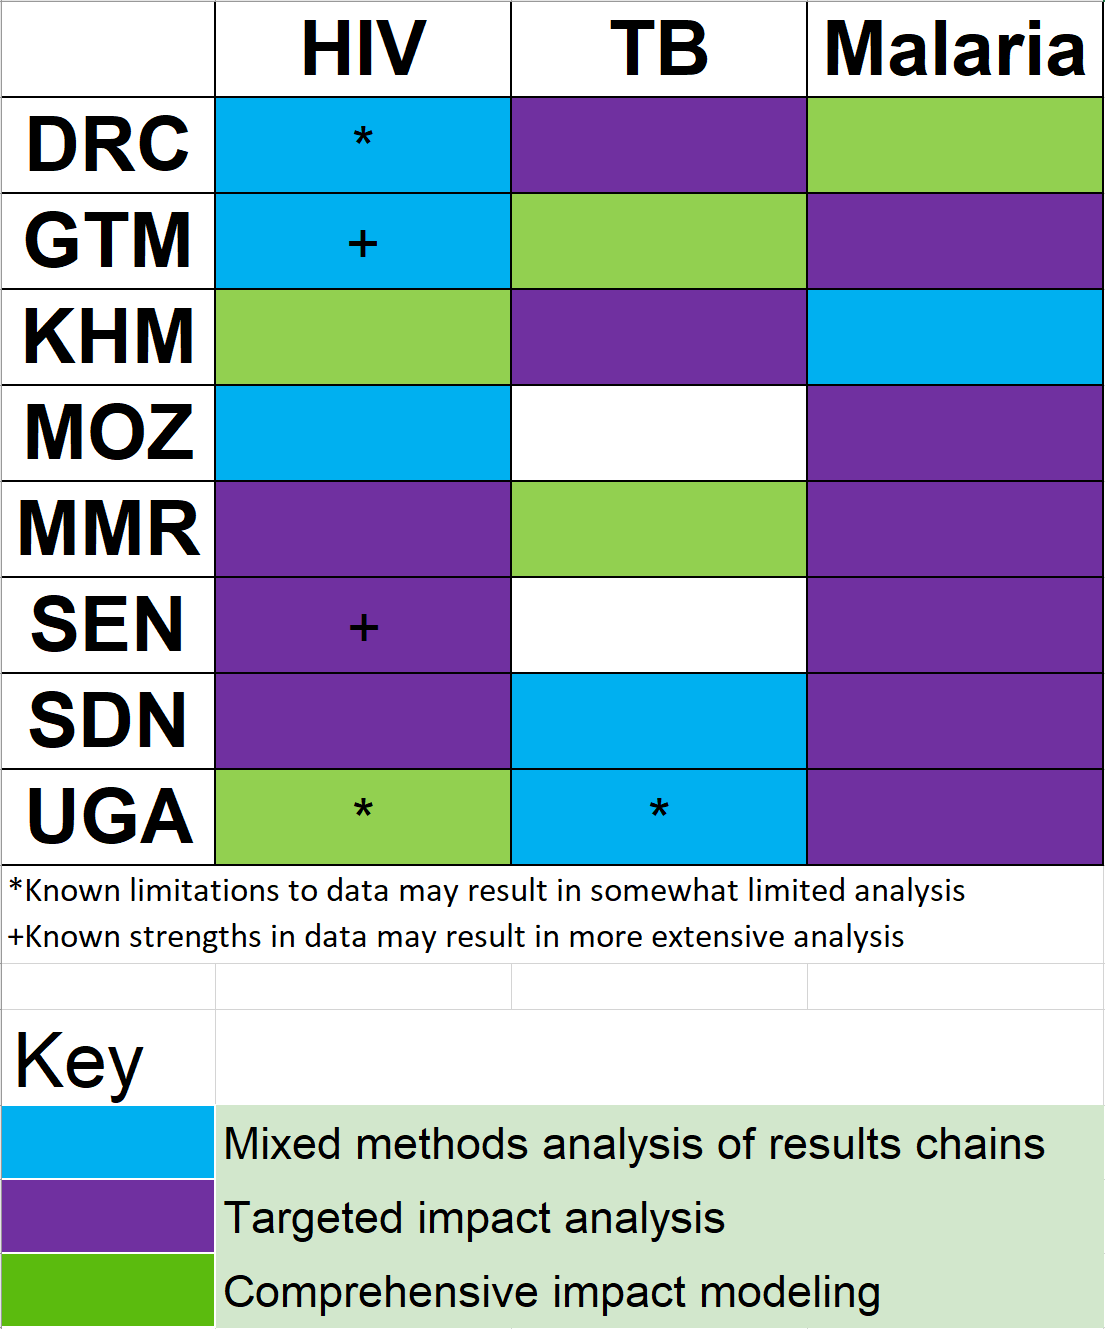
\includegraphics[scale=.4]{Differentiated_Plans_Image.png} \\
  \label{fig1}
\end{figure}


% ------------------------------------------------------------------------------
% Why
\section{Motivation for Differentiated Approaches} \label{why}

There are several reasons why the PCE has opted to take a different approach by diease and country. First and foremost is in an effort to provide results that are relevant to the broad array of audiences who the results might reach. While an overall assessment of the steps leading from Global Fund investment to impact may be relevant and useful to stakeholders in the Global Fund Secretariat, a more tailored analysis focused on isolated sections of the results chains may be more useful to national programs. \\

Second is the feasibility of adding value through impact evaluation. Differences in data availability (indicators tracked and level of disaggregation), data quality, and basic differences in epidemiology limit our ability to apply a generic approach to all diseases in all countries. Furthermore, extensive impact evaluation has already been (or is being) conducted by other organizations for certain diseases in certain countries. For these reasons, the PCE seeks to evaluate different diseases in different ways in order identify applications of existing data that are both possible given known limitations and actually useful to stakeholders. \\

% ------------------------------------------------------------------------------
% Basic Outputs Model
\section{Dose-response model}
STOPPED HERE
% the form of the model
The central model for measuring the contribution of Global Fund inputs to health systems outputs is a structural equation model. The precise functional form of the model and variables in it will be selected to be fit-for-purpose given the output data. In theory, the characteristics of typical output data are that they are integer (whole numbers), over-disbursed (requiring both a mean and variance parameter to describe their distribution), heteroskedastic (different variance at different levels of a given explanatory variable), and temporally-autocorrelated (similar to itself in previous time points). For these reasons, the model is (arguably) most appropriately fit as a generalized linear mixed model (GLMM) in the negative binomial family. For simplicity, I will avoid model notation that explicitly represents a negative binomial GLMM, in order to focus attention on the variables and the level at which they're measured (i.e. indexed). \\

% principle of the model
Measurement of the Global Fund contribution to outputs will rely on the co-variance of outputs and expenditure along three dimensions: space, time and activity. In other words, investments by the Global Fund focus on different interventions in different places, and change from year to year, and so do outputs. If the hypothesis being tested is correct, we would expect to observe changes in health systems outputs that coincide with changes in investments along those three dimensions (space, time and activity). As noted already, the coincidence between changes in outputs and changes in investments alone is not expected to reflect the Global Fund's contribution, but rather the coincidence that happened apart from the correlation that other resources and burden of disease have with outputs. That implies the following regression:

% the model
\begin{equation} \label{basic_model}
O_{jti} = \beta_1 E^{gf}_{jti} + \beta_2 E^{\neg gf}_{jti} + \beta_3 I_{jt}
\end{equation}

% explanation of notation
In this formula, $j$ indexes subnational areas (provinces/ departments, districts/municipalities or otherwise), $t$ indexes time (years, quarters, or months) and $i$ indexes intervention categories, as defined by the Global Fund's Modular Framework. $O$ represents counts of health systems outputs, $E$ represents expenditure either by the Global Fund ($^{gf}$) or other sources ($^{\neg gf}$), and $I$ represents incidence of the disease for which interventions were designed. The $\beta$ terms are coefficients (correlations) to be estimated from the data using maximum likelihood estimation (or similar). This model will primarily be fit separately by disease.\\

% interpretation
The coefficient $\beta_1$ therefore measures the correlation between Global Fund investment and outputs, controlling for other investments and disease burden. Under the assumptions of the PCE Theory of Change and Impact Frameworks (detailed elsewhere), this correlation represents the contribution of the Global Fund to those outputs. \\

% additional considerations
The model as listed in equation \ref{basic_model} estimates only one coefficient relating Global Fund inputs to outputs. In reality, some investments produce more outputs per dollar than others. Features can (and probably will) be added to this model to allow $\beta_1$ to vary by intervention, for example by including a random effect on intervention as an additional parameter in the model. Country-level random effects can also easily be added to allow different estimates of $\beta_1$ between countries, which is likely to also reflect reality more realistically. \\

Note that there are many drivers of $O$ besides $E$ and $I$ that are not included in model \ref{basic_model}, for example cultural context and its relationship with uptake of certain interventions. I argue that the absence such other factors does not bias the estimate of $\beta_1$ because they fall along the causal pathway leading from $E$ to $O$. In other words, the many omitted drivers of $O$ do not influence $E$; they merely dictate why $\beta_1$ is high or low, and therefore are acceptable to exclude from the model. To put this another way, only variables (such as $I$) that are theorized to directly influence both $E$ and $O$ need to be included in the model \ref{basic_model}.

% extension to RSSH
\subsection{Extension to RSSH}
In evaluating the contribution of catalytic and system-wide Global Fund investments (such as investments to strengthen resilient and sustainable systems for health (RSSH)), an additional layer of controls may be necessary. This is because such investments are intended to operate in addition to, or synergistically with, other program areas, not to result in outputs on their own.[CITE] % CITATION NEEDED
 Essentially, this amounts to controlling for Global Fund spending from programs other than just RSSH as well:

% RSSH model
% \begin{equation}
  \begin{align}
    O_{jti} = \beta_1 E^{^{RSSH}}_{jti} + \beta_1 E^{^{HIV/TB/Malaria}}_{jti} \\
    + \beta_2 E^{\neg gf}_{jti} + \beta_3 I_{jt}
  \end{align}
% \end{equation}

% note about using budget as an ITT
\textit{Technical Note: Although expenditure from the Global Fund is the intervention of interest, the above model will also be explored using the approved budget as a proxy for expenditure. The rationale for doing so is to avoid potential bias from differential absorption. Similar to the ``intent to treat'' principle from a randomized control trial, the drivers of actual execution of funds are more diverse and poorly-understood than the drivers of planned budgeting, and thus more challenging to control. To measure the correlation between actual expenditure and outputs would also be to measure the contribution of those absorption-driving factors, and would weaken the interpretability of the coefficient of interest. While both budget and expenditure will be explored, budget will be considered the primary explanatory variable.}


% ------------------------------------------------------------------------------
% Further Details on Model-Based Geostatistics
\section{Relationship with Value for Money} \label{vfm}
The basic outputs model has a natural relationship with value for money (VfM) assessment. As defined by the Global Fund Monitoring and Evaluation team, the key metric of VfM is cost per output, or cost per case averted. [CITE] \\
% CITATION: Briefing
% Strategic Information Department Briefing
% 2017-2022 Strategic KPI Framework Performance targets for KPIs 1, 2 & 8
% March 2018. The Global Fund

The definition of the coefficient $\beta_1$ in formula \ref{basic_model} is the average observed increase in outputs per unit increase in expenditure. $\beta_1$ is also simply stated as the inverse of cost per output (i.e. $cost\, per\, output = \frac{1}{\beta_1}$). In this way, the core model for impact evaluation is the same as the core model for VfM assessment. \\

The key to using the impact evaluation model for VfM assessment is additional interpretation of it. As allocation efficiency is among the critical topics for the PCE, estimates from the core model can be produced among counterfactual scenarios, comparing alternate mixes of interventions and their expected relationship with output. \\

\textit{All sections after this point are intended merely to provide deeper explanation into the topics already presented.}

\bibliographystyle{bmc-mathphys} % Style BST file (bmc-mathphys, vancouver, spbasic).
\bibliography{bmc_article}      % Bibliography file (usually '*.bib' )

\end{backmatter}

\end{document}
